
\documentclass[12pt,a4paper]{scrartcl}		% KOMA-Klassen benutzen!

\usepackage[ngerman]{babel}			% deutsche Namen/Umlaute
\usepackage[utf8]{inputenc}			% Zeichensatzkodierung
\usepackage{graphicx}				% Einbinden von Bildern
\usepackage{color}				% Farben wenn es sein muß
\usepackage{amsmath}		
\usepackage{amsfonts}
\usepackage{listings}

\definecolor{codegreen}{rgb}{0,0.6,0}
\definecolor{codegray}{rgb}{0.5,0.5,0.5}
\definecolor{codepurple}{rgb}{0.58,0,0.82}
\definecolor{backcolour}{rgb}{0.95,0.95,0.95}

\lstdefinestyle{mystyle}{
    backgroundcolor=\color{backcolour},   
    commentstyle=\color{codegreen},
    keywordstyle=\color{magenta},
    numberstyle=\tiny\color{codegray},
    stringstyle=\color{codepurple},
    basicstyle=\ttfamily\footnotesize,
    breakatwhitespace=false,         
    breaklines=true,                 
    captionpos=b,                    
    keepspaces=true,                 
    numbers=left,                    
    numbersep=5pt,                  
    showspaces=false,                
    showstringspaces=false,
    showtabs=false,                  
    tabsize=2
}

\lstset{style=mystyle}

\newcommand\svthema{INF264 Project 1}
\newcommand\svperson{Sophie Blum and Benjamin Friedl}
\newcommand\svdatum{18.09.2020}
\newcommand\lvname{Implementing decision trees}
\begin{document}

\title{ \svthema}
\author{\textsc{\lvname}}
\date{ \small \textsl{\svperson} --- \svdatum }
\maketitle

\abstract
About the document:
The names behind every function description point put, who initially wrote the code for this functionality. 
The largest amount of time however went into debugging and correcting the code, as well as re-evaluating the 
design choices and making the algorithm work. We did all this together, so that it is hard to point out, who 
did what exactly.

\section{Implementation of the tree data structure (Sophie)}
The decision tree is implemented as a node data structure in a semi-object-oriented way. A tree is viewed as 
a root with children connected to it. That means that every node can be the root of a tree (and every node is 
indeed the root of its subtree). As every node could be a tree, the decision tree is not encapsulated in a 
data structure itself and has to be given as a parameter for every function that uses it (see also: learn())
The nodes themselves are implemented in the node class, which contains variables for data and the majority 
label in the subtree denoted by this node. 
The data variable holds either the feature for the corresponding decision or a label, if the node is a leaf 
in the tree.
The majority label is used for pruning.
The node also has a reference to its parent and its children. The latter are organized in a list of tuples. 
Every tuple has a reference to the child node as well as the value that is used for the decision. 

\begin{lstlisting}[language=Python]
    class node: 
        def __init__(self, data, parent = None, majority_label = None):
            self.data = data
            self.parent = parent
            self.majority_label = majority_label
            self.children = []
        def __str__(self):
            return f"{self.data} - {self.children}"
        def addChild(self, child):
            self.children.append(child)
\end{lstlisting}

The printTree() is an inorder traversal of a tree denoted by a root-node. 
Remark: We designed the data structure before we knew we only had to compute binary trees, so this could have 
been implemented easier by just storing each child node separately and having only one variable to denote the 
decision value.

\section{Implementation of learn (Sophie)}
The learn function is splitted into to separate functions, as the integration of pruning is easier that way. 
In fact the learn\_rec() has been learn() in the first place. As we implemented pruning and needed to integrate 
it, the easiest way was to split the function into two parts.

Learn\_rec() is the powerhouse of the learn function and outputs the root node of the decision tree, that is 
learned on the input data. 
The function first checks all base cases and outputs the majority label as a leaf. 

\begin{lstlisting}[language=Python]
    if same_value(y):
        return node(y[0])
    elif len(X[0]) == len(used_feature_list) or same_value(X):
        label = get_maj_label(y)
        return node(label)
\end{lstlisting}

When there is no base case 
present, a feature gets selected based on the selected impurity measure (separately implemented). To keep track 
of the already used features, the all get appended to an array that is given as a parameter to the function. 
The dataset then gets splitted based on the mean of the selected feature. These separate datasets are then 
used for a recursive call of the same function. All the created nodes get assigned their respective parent 
and/or children.
All this functionality is subdivided in different functions doing smaller tasks.

Learn()  is just the packaging for the recursion and the pruning in one function. It splits the given dataset, 
trains a decision tree with learn and uses pruning afterwards. All of this according to the input, whether 
pruning is wanted or not.

\begin{lstlisting}[language=Python]
    def learn(X, y, impurity_measure, pruning):
        seed = 432
        if(pruning):
            X_train, X_prun, Y_train, Y_prun = model_selection.train_test_split(X, y, test_size= 0.3, shuffle=True,                                                                                 random_state = seed)
        else:
            X_train = X
            Y_train = y
        root = learn_rec(X_train, Y_train, [], impurity_measure)
        if pruning:
            root = pruning_function(root, X_prun, Y_prun)
        return root
\end{lstlisting}

\section{Implementation of the impurity measures (Benjamin)}
Both, entropy as well as the Gini-impurity, need for its calculation only the probabilities of different 
possible values. The latter is computed by the function “probability\_list” which takes a list of numbers 
and first counts the occurrence for all the different values. This is done through a for-loop over all 
elements in the input-list. 

\begin{lstlisting}[language=Python]
    for i in range(count_values):
        if (values[i] not in value_list): 
            value_list.append(values[i])
            prob_list.append(1)
            different_val +=1
        else:
            for j in range(different_val):
                if(values[i]==value_list[j]): prob_list[j]+=1
\end{lstlisting}
 
If the value of the viewed element didn’t occur before, it gets appended to the value\_list while prob\_list 
saves the value 1 at the same index. Else the algorithm searches the index in the value\_list with the right 
value and increments the value in the prob\_list at the right index. 
To get the probabilities, every numbers of occurrence is divided by the total length of the input-list.

\begin{lstlisting}[language=Python]
    for k in range(different_val):
        prob_list[k] = float(prob_list[k]) / count_values
\end{lstlisting}

In order to get the entropy and Gini-impurity, one can first compute this probability\_list and implement 
the summation with a simple for-loop.

\begin{lstlisting}[language=Python]
    def entropy(values):
        prob_list = probabiliy_list(values)
        different_values = len(prob_list)
        sum = 0
        for i in range(different_values):
            sum -= math.log(prob_list[i], 2) * prob_list[i]
        return sum

    def gini(values):
        prob_list = probabiliy_list(values)
        different_values = len(prob_list)
        sum = 0
        for i in range(different_values):
            sum += prob_list[i]*(1-prob_list[i])
        return sum
\end{lstlisting}

\section{Implementation of the decrease in impurity through a split (Benjamin) }
The value of decrease in impurity is computed by the function “information\_gain”, which takes a feature-vector x, 
a label-vector y and a string describing the impurity-measure as input and is implemented in three steps. 
First, the mean value of all values in x is calculated. This is done by a simple for-loop over all values in x.

\begin{lstlisting}[language=Python]
    mean = 0
    count = 0
    for i in range(len(x)):
        mean += x[i]
        count +=1
    mean /= count
\end{lstlisting}

Secondly, the split of the label-vector is realised in two lists “leq\_mean” and “g\_mean” containing all 
values from x less equal or greater than the mean. Additionally, the percentual occurrence of the values 
in “leq\_mean” is computed in “prob\_leq\_mean”.

\begin{lstlisting}[language=Python]
    leq_mean = []
    g_mean = []
    count_leq_mean = 0
    for i in range(len(x)):
        if(x[i] <= mean):
            count_leq_mean +=1
            leq_mean.append(y[i])
        else:
            g_mean.append(y[i])
    prob_leq_mean = count_leq_mean / count
\end{lstlisting}

Lastly the Impurities before and after the split are calculated using the already implemented functions 
“entropy” or “gini”.

\begin{lstlisting}[language=Python]
    f(impurity_measure=="entropy"):
        impurity = entropy(y)
        conditional_impurity = prob_leq_mean * entropy(leq_mean)+ (1-prob_leq_mean) * entropy(g_mean)
    elif(impurity_measure=="gini"):
        impurity = gini(y)
        conditional_impurity = prob_leq_mean * gini(leq_mean)+ (1-prob_leq_mean) * gini(g_mean) 
    else:
        print("Not known impurity measure")

\end{lstlisting}

Using that, the function returns the value of decrease in impurity through the split, which is the 
information gain in the case of entropy.
 
\begin{lstlisting}[language=Python]
    return impurity - conditional_impurity
\end{lstlisting}

\section{Implementation of predict (Benjamin)}
This function gets as parameter a vector x and returns the predicted label. Generally, it is implemented as 
recursion starting with the root and then continuing with the child for which the value of x at the looked 
at feature fits. 
If the (sub-)tree is a leaf, that is when the (sub-)tree’s children-list is empty, then the function returns 
the label memorized in node.data. 

\begin{lstlisting}[language=Python]
    if (not node.children):
        return node.data
\end{lstlisting}
 
Otherwise, a for loop goes through the children-list, which is sorted by the value of split. In the case of 
a binary split, there is only one split point, so in children[0][1] and children[1][1] there is both times 
memorized the mean-value. 
Furthermore, if the value of the feature-vector at the splitting feature, which memorized as index in node.data 
for not-leaf nodes, is less than the mean value, then we recursively call predict for the child-node memorized 
in children[i][0]. 

\begin{lstlisting}[language=Python]
    if(x[node.data] < node.children[i][1]):           
            return predict(node.children[i][0],x) 
\end{lstlisting}

If we reached the end of the children-list, it means the vector at the looked upon feature has a higher value 
than every splitting point and we recursively call predict for the last child-node. 

\begin{lstlisting}[language=Python]
    elif(i==count_values-1):                    
            return predict(node.children[i][0], x)
\end{lstlisting}

Remark: We implemented this function before we knew we only had to compute binary trees, so this could have 
been implemented easier by just looking at the left and right child.

\section{Implementation of pruning (Benjamin)}
The pruning-function takes as input a node representing a (sub-)tree and the pruning data X\_prun and y\_prun. 
It returns a node representing the post-pruned input-tree. 
First, the pruning function searches the leafs of the decision tree. Therefore, it recursively calls itself 
until the length of the children-list is not zero. 

\begin{lstlisting}[language=Python]
    if (len(node.children)!=0):  
        for i in range(len(node.children)):
                #call recursion on each child
                pruning_function((node.children[i])[0], X_prun, y_prun) 
    else:
        #reached leaf
        return node
\end{lstlisting}

Afterwards, it goes back up the tree and checks for every node whether the accuracy of the (sub-)tree on the 
pruning-data is lower than the accuracy when predicting the majority label. 
In this case, we change the node into a leaf predicting the majority label. 

\begin{lstlisting}[language=Python]
    if (acc(node, X_prun, y_prun) < majority_label_acc(node.majority_label, y_prun)):
        node.data = node.majority_label
        node.children = []
    return node
\end{lstlisting}

The accuracies are implemented through a simple for-loop counting the right predictions. 

\begin{lstlisting}[language=Python]
    def majority_label_acc(majority_label, y_prun):
        x = 0
        for i in range(len(y_prun)):
            if(y_prun[i]==majority_label):
                x += 1
        return float(x) / len(y_prun)

    def acc(node, X, Y):
        x = 0
        for i in range(len(Y)):
            if(Y[i]==predict(node, X[i])):
                x += 1
        return float(x) / len(Y)
\end{lstlisting}

\section{Evaluation (Benjamin, Sophie)}
First, we split the Data into Training-, Evaluation and Test-data. 

\begin{lstlisting}[language=Python]
    seed = 111
    X_train, X_val_test, Y_train, Y_val_test = model_selection.train_test_split(X, y, test_size= 0.3, shuffle=True, random_state = seed)
    seed = 112
    X_val, X_test, Y_val, Y_test = model_selection.train_test_split(X_val_test, Y_val_test, test_size= 0.5, shuffle=True, random_state = seed)
\end{lstlisting}

We chose a ratio of 0.7, 0.15, 0.15 to have sufficient training-data whilst getting representative accuracies. 
Afterwards we implemented four trees, one for each impurity measure with and without pruning and computed the 
accuracy on the training- as well as validation-data. This example shows one the procedure for the tree using 
entropy and pruning. 

\begin{lstlisting}[language=Python]
    tree_ent_prun = learn(X_train, Y_train, impurity_measure="entropy", pruning=True)
val_acc_ent_prun = acc(tree_ent_prun, X_val, Y_val)
train_acc_ent_prun = acc(tree_ent_prun, X_train, Y_train)
\end{lstlisting}

We got the following results: 

\begin{figure}[h]
    \centering
    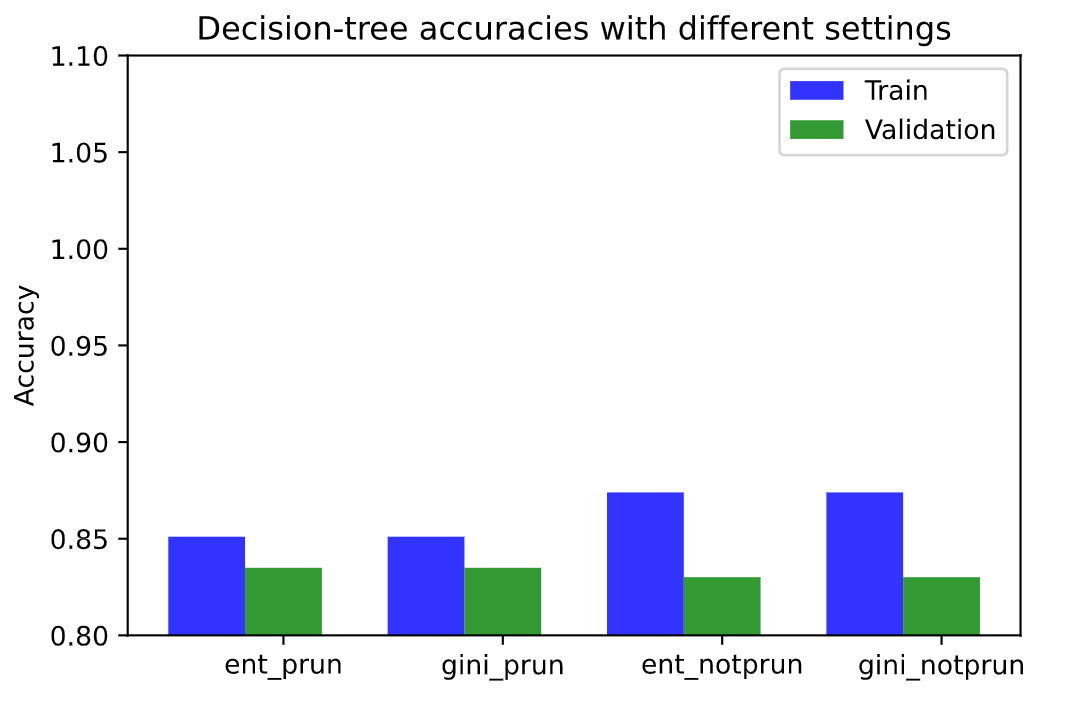
\includegraphics[scale = 0.8]{results.png}
    \caption{Results}
\end{figure}

The accuracies of the trees don’t change for the different impurity measures. Moreover not using pruning, 
the training-accuracy is higher than the validation-accuracy, which was expected as it is susceptible to 
overfitting. As the validation-accuracy is higher using pruning, we decided to use the tree trained by using 
entropy and pruning.

\section{Testing (Benjamin, Sophie)}
We now tested the chosen tree to get a representative estimate of the accuracy. 

\begin{lstlisting}[language=Python]
    test_acc = acc(tree_ent_prun, X_test, Y_test)
\end{lstlisting}

The test-accuracy was with 0.9515 lower than the according training- and validation-accuracy. Nevertheless, 
the difference was less than 1.6\% and a slightly lower test-accuracy is to be expected as we used the other 
accuracies to choose this tree.  

\section{Comparison to existing implementations (Sophie)}

\end{document}